\subsection{实验目的}
理解遥感图像分类的概念,掌握一些典型的图像无监督分类方法,例如K均值聚类算法。完成遥感图像的图像分类。
\subsection{实验原理}
\begin{figure}[H]
	\centering
	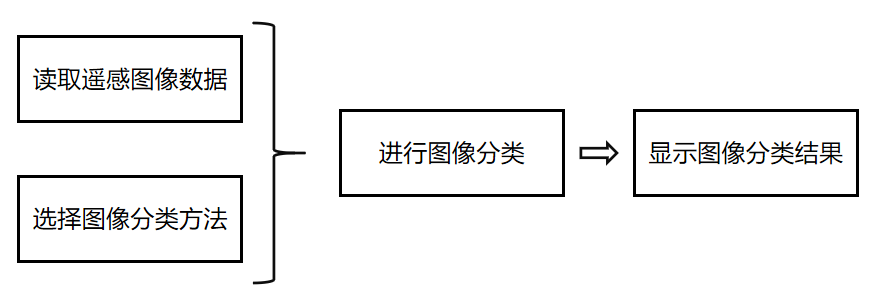
\includegraphics[width=0.7\linewidth]{figure/classification_flowchart.png}
	\caption{进行图像分类的步骤}
\end{figure}
\subsubsection{图像分类的概念}
将图像中的像素点划分为不同的类别,每一个类别具有特定的物理含义。例如不同的地物类型,包括草地、水泥地、建筑、道路、森林、山地等。

图像分类的两个步骤:特征提取和分类算法。
\begin{description}
	\item[特征提取] 如何描述每一个像素点,颜色特征向量。
	\item[分类算法] k均值据类算法。
\end{description}
\subsubsection{k均值聚类算法}
k均值据类算法是一个迭代算法,迭代更新每一个类别的聚类中心,并且通过最近邻准则完成分类。
\begin{description}
	\item[算法描述] \begin{enumerate}
		\item 任选K个初始聚类中心:$Z_1(1)$,$Z_2(1)$,$\dots$,$Z_K(1)$
		\item 按最小距离原则叫其余样本分配到K各聚类中心中的某一个,即
		\[ \text{若} \min\left\lbrace \left\| \mathbf{X}-\mathbf{Z}_i(k) \right\|,i=1,2,\dots,K \right\rbrace=\left\| \mathbf{X}-\mathbf{Z}_j(k) \right\|=D_j(k) \]
		则$X\in S_j(k)$
		\item  计算各个聚类中心的新向量值:$\mathbf{Z}_j(k+1)\quad j=1,2,\dots,K$
		\[ \mathbf{Z}_j(k+1)=\frac{1}{N_j}\sum_{\mathbf{X}\in S_j(k)}\mathbf{X}\quad j=1,2,\dots,K \]
		\item 如果$\mathbf{Z}_j(k+1)\neq\mathbf{Z}_j(k)\quad j=1,2,\dots,K$,则回到2,将模式样本逐个重新分类,重复迭代计算。
		
		如果$\mathbf{Z}_j(k+1)=\mathbf{Z}_j(k)\quad j=1,2,\dots,K$,算法收敛,计算完毕。
	\end{enumerate} 
\end{description}
\subsection{实验流程}
\begin{figure}[H]
	\centering
	\begin{tikzpicture}[node distance=1.5cm]
	\node(start) [startstop] {开始};
	\node(input_img) [io, below of=start] {输入待分类的图像};
	\node(radom_center) [process, below of=input_img] {随机选取聚类中心};
	\end{tikzpicture}
\end{figure}
\subsection{实验程序}
\lstinputlisting[caption={K均值聚类程序}]{"../Executable Script/Exp 4/ReadAirportImages.m"}
\subsection{实验结果和分析}